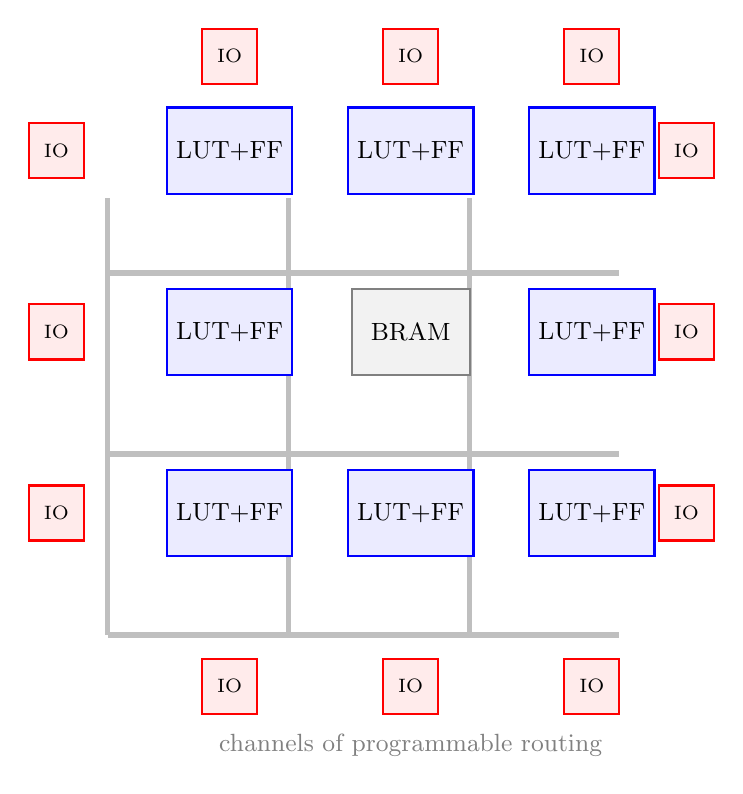
\begin{tikzpicture}[x=1cm,y=1cm,
  clb/.style={draw=blue, thick, fill=blue!8, minimum width=1.5cm, minimum height=1.1cm, font=\small},
  blk/.style={draw=gray, thick, fill=gray!10, minimum width=1.5cm, minimum height=1.1cm, font=\small},
  iob/.style={draw=red, thick, fill=red!8, minimum width=0.7cm, minimum height=0.7cm, font=\scriptsize}]
% routing channels
\foreach \x in {0,2.3,4.6} {\draw[gray!50, line width=2pt] (\x-0.95,-0.95) -- (\x-0.95,4.6);}
\foreach \y in {0,2.3,4.6} {\draw[gray!50, line width=2pt] (-0.95,\y-0.95) -- (5.55,\y-0.95);}
% CLB grid
\node[clb] at (0.6,0.6) {LUT+FF}; \node[clb] at (2.9,0.6) {LUT+FF}; \node[clb] at (5.2,0.6) {LUT+FF};
\node[clb] at (0.6,2.9) {LUT+FF}; \node[blk] at (2.9,2.9) {BRAM};  \node[clb] at (5.2,2.9) {LUT+FF};
\node[clb] at (0.6,5.2) {LUT+FF}; \node[clb] at (2.9,5.2) {LUT+FF}; \node[clb] at (5.2,5.2) {LUT+FF};
% IO ring
\foreach \p in {(0.6,-1.6),(2.9,-1.6),(5.2,-1.6),(-1.6,0.6),(-1.6,2.9),(-1.6,5.2),(0.6,6.4),(2.9,6.4),(5.2,6.4),(6.4,0.6),(6.4,2.9),(6.4,5.2)} \node[iob] at \p {IO};
\node[gray, font=\small] at (2.9,-2.35) {channels of programmable routing};
\end{tikzpicture}
